
\chapter{Design and Verification}

Compass is a tool is used to analyze software (both source code and binaries). 
A collection of {\em checkers} are build with each of them detecting the 
violation of a rule.  By reporting on the violations of rules {\em Compass} provides 
a way to enforce predefined or arbitrary user specified properties on software.
This chapter covers the design of {\em Compass} and the design of the verification in 
the \emph{Compass Verifier}, used to verify properties of the checkers implemented 
and submitted to {\em Compass}.

% \section{Use Cases}
\section{Usage Model}

\label{design::UseCase}

Figure~\ref{Compass_usecase} shows the usage model (use cases) of \emph{Compass}.
The analysis is triggered by the user running {\em Compass} over an
input file (source code or binary). The user implicitly selects 
which checkers to execute (defining what rules are to be enforced); 
by default all checkers are run. 
The user also specifies the input file to be checked; for source code 
the specification is similar to the command line required for the 
compilation in the case of a source file.  Results of the analysis 
are presented to the user, a number of mechanisms can be used to 
display the results.

\begin{figure}[th]
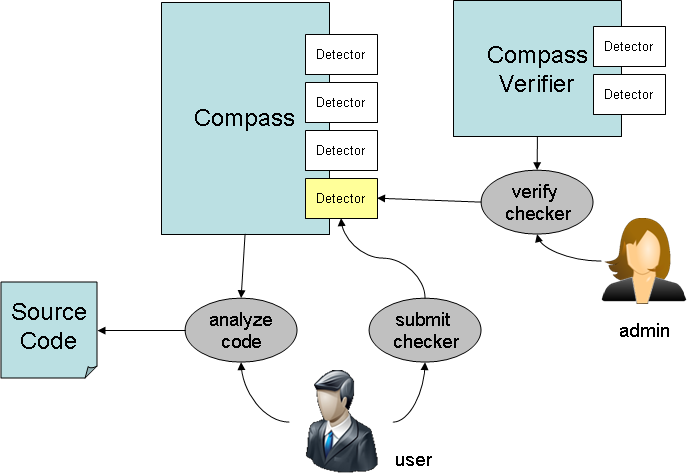
\includegraphics[width=4.5in]{compass_pic.png}
\caption{Compass Use Case}
\label{Compass_usecase}
\end{figure}

Either the same user or a different user/developer can also
implement and submit checkers to be built into Compass.
% Furthermore, a user may contribute with his own checkers that can be added to Compass. 
Since external users may contribute checker automatically via scripts, a verification of the 
validity and safety of these checkers is necessary. We provide a \emph{Compass Verifier}
that helps to check that all checkers are safe. Currently, the verifier is run by
an administrative person but may run automatically in the future.

%\section{Assumption of trust} 
\section{Trust Model}
By design we make a few assumptions about the use of Compass in order to define
a secure tool. We assume:
\begin{enumerate}
   \item For now, there is an assuption of trust in the person writing the checker. \\
      We use the \emph{Compass Verifier} as a way to double check the 
      checkers so that we can eventually weaken the level of trust assumed for people 
      writing checkers. However, the design of the \emph{Compass Verifier} is not likely to
      ever be robust enough to guarantee an automated proof of security for each checker.  
      Thus, we also assume that someone trusted will also review the checker.
      {\em not implemented: We expect that a digital signature is possible to associate 
      a trusted reviewer with a review of the checker together with an MD5 hash that
      verifies the checker source code.}

   \item Since running \emph{Compass Verifier} is an optional part of building 
      the Compass executable, the person running these test is trusted. There are
      two ways to run the \emph{Compass Verifier} (see section \ref{sec:compass_verify}
    for details):
      \begin{itemize}
         \item Slow: once on each checker ({\tt make verify}). This mechanism
            tests all the files one checker at a time and thus can not miss 
            a file.  Note that even the counter examples are tests which can 
            be a problem when the counter example for the checker is detected
            as a violation for \emph{Compass Verifier}.  Conter examples for
            checkers have to be carefull written to not represent examples that
            violate \emph{Compass Verifier}.
         \item Fast: once on the union of all the checkers ({\tt make oneBigVerify}).
            This step forms a single file of all the checkers (and indoing so can
            miss some files, and so is less secure).  It is mostly for testing 
            purposes.
      \end{itemize}

   \item The person building the Compass executable is trusted.

   \item The environment where the testing using Compass is done is trusted.

   \item Compass is designed so that the user running Compass need not be trusted.

\end{enumerate}

It is unclear at present how weak the assumption of trust on the compass checker developer 
can be and it may ultimately depend directly on the capabilities of the \emph{Compass Verifier}.


\section{Architecture}

\begin{figure}[thb]
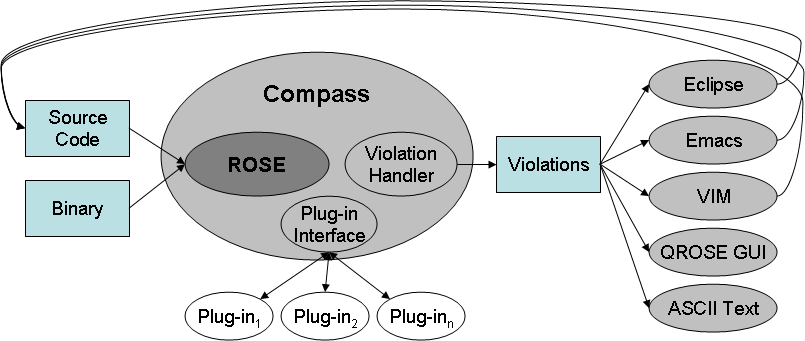
\includegraphics[width=6.0in]{compass_arc.png}
\caption{Compass Architecture}
\label{CompassArchitecture}
\end{figure}


Compass is a tool that allows users to implement checkers to locate and
report software defects.
Documentation of various kinds of software defects can be found in sources
such as the CERT Secure Coding Rules, Common Weakness Enumeration from MITRE, 
and other sources. Our focus is not to define new software defects but
rather to provide a platform that allows the easy implementation of defect
checkers.  Compass has been designed to be easy to extend, allowing users to 
implement their own custom checkers (custom source code analyses for
identifying defects), as shown in Figure~\ref{CompassArchitecture}. Compass supports
the implementation of both simple as well as more advanced defect
checkers. For the latter, Compass utilizes the ROSE infrastructure to
perform a wide range of general purpose program analyses, such as control
flow analysis, data flow analysis, program slicing, etc.


Compass is designed in a way that allows users who do not necessarily have
compiler backgrounds to utilize the ROSE infrastructure to build their
own analysis tools.
Compass is foremost an extensible open source infrastructure for the
development of large
collections of rules. Our current implementation supports automatic
defect checking, programming language restriction, and malware detection in
C, C++, and object code.
Support for Fortran is a new addition to ROSE and will be supported in
Compass in the near future.




\section{Design}

\begin{figure}[thb]
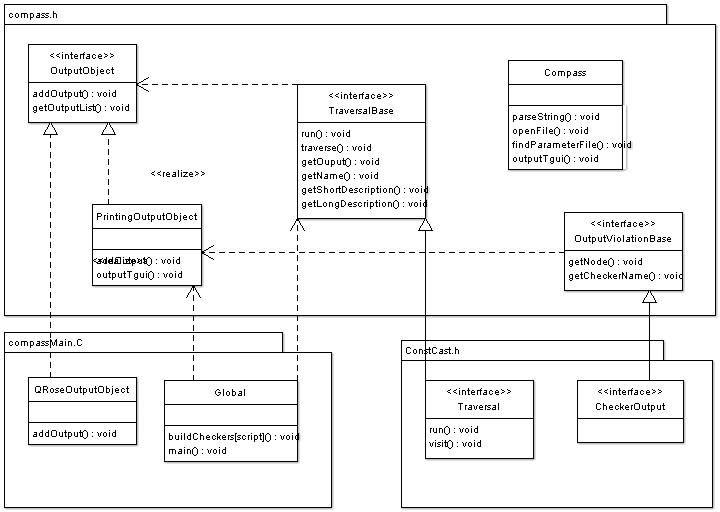
\includegraphics[width=6.0in]{compassdesign.png}
\caption{Compass Design}
\label{CompassDesign}
\end{figure}

Compass is designed to be easy to extend. Any user may write a checker and add it to
Compass. Figure~\ref{CompassDesign} illustrates the UML design decisions behind Compass.


Most of the functionality of Compass is in abstract classes hidden in the Compass
namespace within compass.h - a file within the compassSupport directory. The figure uses a
specific example, {\em ConstCast}, for illustration; Compass is designed to support a large
number of checkers (hundreds). All checkers, such as the {\em ConstCast} checker (illustrated in
figure~\ref{CompassDesign}), utilize the abstract classes to traverse a program with all
its nodes and to output violations found in that code according to the local algorithm.

CompassMain is the main executable that initially calls ROSE to parse a program. Then
\emph{buildCheckers} is called to load all checkers that are specified within a
configuration file. The configuration file allows users to turn on and off specific
checkers for their run-time analyses. However, the configuration file only permits
checkers to be loaded that were part of Compass at compile-time.

The main interface file compass.h contains the abstract classes \emph{TraversalBase} and 
\emph{OutputObject}. TraversalBase is the interface to ROSE, allowing a checker to
traverse the ROSE AST (program) and hence perform analysis on that AST. OutputObject aids
to output defects found by a specific checker. More functionality to handle e.g. file
input and parameters provided to Compass, is provided within the Compass namespace.

\section{Compass Verifier}

Compass must be safe, so that analyses and their results can be trusted. 
The {\em Compass Verifier} is used at build time to run a specific set of separate 
compass rules offer the source cod eof all the checkers.  For simplicity it runs in two
modes: fast, for checking specific named checker source files; and slow, for testing 
{\em all} checker source files.

\subsection{Threats} 

In order to define a complete design for security we outline the threats that
understand to be relevant. The main threats to the validity of Compass checkers are:
\begin{itemize}
\item \emph{Malicious User} \\ 
  A malicious user is an external user of Compass contributing a checker that performs malicious behavior.
\item \emph{Malicious Checker} \\ 
  Compass is extensible and new checkers can be added externally (users outside the main development group).
  A checker can be programmed arbitrarily using the C/C++ and assembly programming languages. 
  It is therefore possible for a skilled programmer to hide malicious operations within a
  checker.  Compass must prevent checkers with malicious behavior to be part of the
  Compass system. Threats are:
   \begin{itemize}
      \item {\bf exfiltration} \\
         A checker should act in a secure way with the input files it is given.
         Securing the inputs to Compass (e.g. the inputs to each checker) from 
         exfiltation is a first priority. Allowing a checker to scan the host 
         machine to exfiltrate arbitrary data (this is a threat that any secure
         software will have).
      \item {\bf modification of filesystem} \\
         A checker should be side-effect free, or have only well defined side-effects, 
         but a malicious checker could modify or erase parts of the accessible file 
         system (e.g. deleting whole directory structures).
%     \item {\bf others ??? ...}
   \end{itemize} 

\item \emph{Malicious Compass} \\
    Since Compass is built from ROSE, it is possible to modify compass (or any checker) 
    to generate source code that could be compiled to replace the existing executable
    (there are some constraints here) or regenerate the source code to replace the 
    existing source code or perhaps just provide an alternative copy of the source code.
    This indirect transformation of the input code is a threat.

\item \emph{Source Code Replacement} \\ It should not be possible for users to exchange the
    source code of checkers within a running system, i.e. Compass cannot implement dynamic
    loading of checkers. Such a feature would compromise its safety.

\item \emph{Binary Replacement} \\ Another threat is the replacement of a valid Compass
    checker with a modified malicious version within a binary release of Compass.
    Therefore, Compass should be aware if parts of itself were modified and should not
    execute.

\end{itemize} 

%\subsection{Safety Handling}
\subsection{Mitigation of Threats}

Compass is designed to be safe. The Compass Verifier is a stable separate copy of Compass
that contains only a few checkers to check (external and internal) user delivered checkers
for safety.  We have hopefully designed Compass in a way that it addresses the threats
mentioned above:
\begin{itemize}
\item \emph{Malicious User} \\ Initially, we permit only trusted individuals to add new
    checkers to Compass. Once the verification process is matured, we will extend this
    policy to allow less trusted users to contribute to Compass. A goal will be to allow
    arbitrary users to contribute checkers, however, a review of the whole Compass design
    (and the {\em Compass Verifier} especially) will be required to define required trust
    levels for user/developers who implement checkers.
\fixme{We might define trusted and untrusted checkers as a way to have checkers from
       arbitrary users, but mark them as untrusted.}

\item \emph{Malicious Checker} \\ To prevent Compass from executing malicious code, the Compass
    Verifier executes its own checkers on any user defined checker that is being
    considered to be added to Compass. Currently, the Compass Verifier contains three checkers:
   \begin{itemize}
      \item \emph{fileReadOnlyAccess} ensures that a user defined checker performs no write
         or execute operations on files.
      \item \emph{forbiddenFunctions} is a {\em white list} of function calls permitted in
\fixme{Change to allowed functions?}
         a checker. This list contains functions that are trusted and hence considered
         unharmful when integrated to Compass.
      \item \emph{noAsmStmtsOps} searches for assembly instructions in a checker and flags
         and reports all cases as unsafe.
      \item To avoid modifications of the AST for the purpose of allowing other checkers
         to pass, the AST should not be modified (this should extend to all the
         program analysis graphs generated and used by other checkers).
         {\em This is not implemented yet.} 
\end{itemize}

\item \emph{Malicious Compass} \\
    Since Compass does not generate code, it can not be used to modify the input software
    (source code or binary) or generate an new copy that could be confused with the input.
    However, future versions of Compass make make transformation to introduce greater
    levels of security; fix flaws, mitigate specific forms of threats, etc.  It will be
    important to make sure that such transformation can not change the behavior of an
    input code to make the modified input code malicious.  Current proposed approaches
    would build a patch which would have to be inspected by a trusted developer before
    it would be applied to modify the input code.

\item \emph{Source Code Replacement} \\ Checkers can only be added at compile time to
    Compass, not at run-time. This means that checkers (meaning the source code) cannot be
    exchanged against unsafe versions at run-time. Furthermore, we allow only the Compass
    tool builder (admin) to build versions of Compass that must pass the Compass Verifier.

\item \emph{Binary Replacement} \\ Our goal is to perform a MD5 checksum on all the checkers
    part of the binary Compass distribution before Compass is executed. In this way
    Compass will not run if parts of it were modified. {\em This is not implemented yet.}
\fixme{We should describe the policy for allowing MD5 checksums to be verified.}

\end{itemize} 


%The above list contains an important subset of checkers that enforce Compass checkers to be safe. 
%Additional checkers can easily be added to that list.
%In the future, a checker submitted to Compass, should go first through the automatic verifier, before it is either 
%added to Compass or denied.  


